\placelogofalse
\begin{frame}{Moments}
\begin{columns}
\column{0.48\linewidth}
\begin{center}
\begin{outline}
\1 Capture integral properties of mass density field
\2 Project onto polynomial basis, $b_i$
\end{outline}
\end{center}

\column{0.48\linewidth}
\begin{center}
  \textbf{Moment}
  $$
  M_{i,j,k} = \int_{\Omega} x^i y^j z^k \rho d\Omega
  $$
  Where $i, j, k \in \{0, 1, 2, \cdots\}$

  \vspace{1.5cm}

  \textbf{Moment Vector}
  \begin{align*}
    \bf{M} &= [M_{0,0,0}, M_{1, 0, 0},\\
      & \cdots, M_{n, 0, 0}, M_{n, 1, 0},\\
      & \cdots, M_{n, n, 0}, M_{n, n, 1},\\
      & \cdots, M_{n,n,n}]^T
  \end{align*}
\end{center}
\end{columns}
\end{frame}
\placelogotrue

\begin{frame}{Quadrature From Moments}
We can approximate an integrand f with weighted basis functions.
$$
f \approx \sum_{i = 1}^n c_i b_i
$$
Then by linearity of integrals
$$
\int_{\Omega} f d\Omega \approx \int_{\Omega} \sum_{i = 1}^n c_i b_i \ d \Omega
= \sum_{i=1}^n c_i \int_{\Omega} b_i \ d \Omega
$$
Where $m_i = \int_{\Omega} f_i d \Omega$
\end{frame}

\begin{frame}{Moment Fitting for Quadrature Rules}
\centering
\begin{center}
$$
\bf{A} \cdot \bf{W} = \bf{M}
$$
Where
$$
\bf{A} = \left[
\begin{array}{cccc}
  b_1(x_1) & b_1(x_2) & \cdots & b_1(x_q) \\
  b_2(x_1) & b_2(x_2) & \cdots & b_2(x_q) \\
  \vdots & \vdots & \ddots & \vdots \\
  b_n(x_1) & b_n(x_2) & \cdots & b_n(x_q) \\
\end{array}\right],
W = \left[
  \begin{array}{c}
    w_1 \\ w_2 \\ \vdots \\ w_q
  \end{array}
\right],
M = \left[
  \begin{array}{c}
    m_1 \\ m_2 \\ \vdots \\ m_q
  \end{array}
\right],
$$
With $m_i = \int_{\Omega} b_i \ d\Omega$
\end{center}
\end{frame}

\begin{frame}{Compress Quadrature}
  \centering
  \begin{center}
    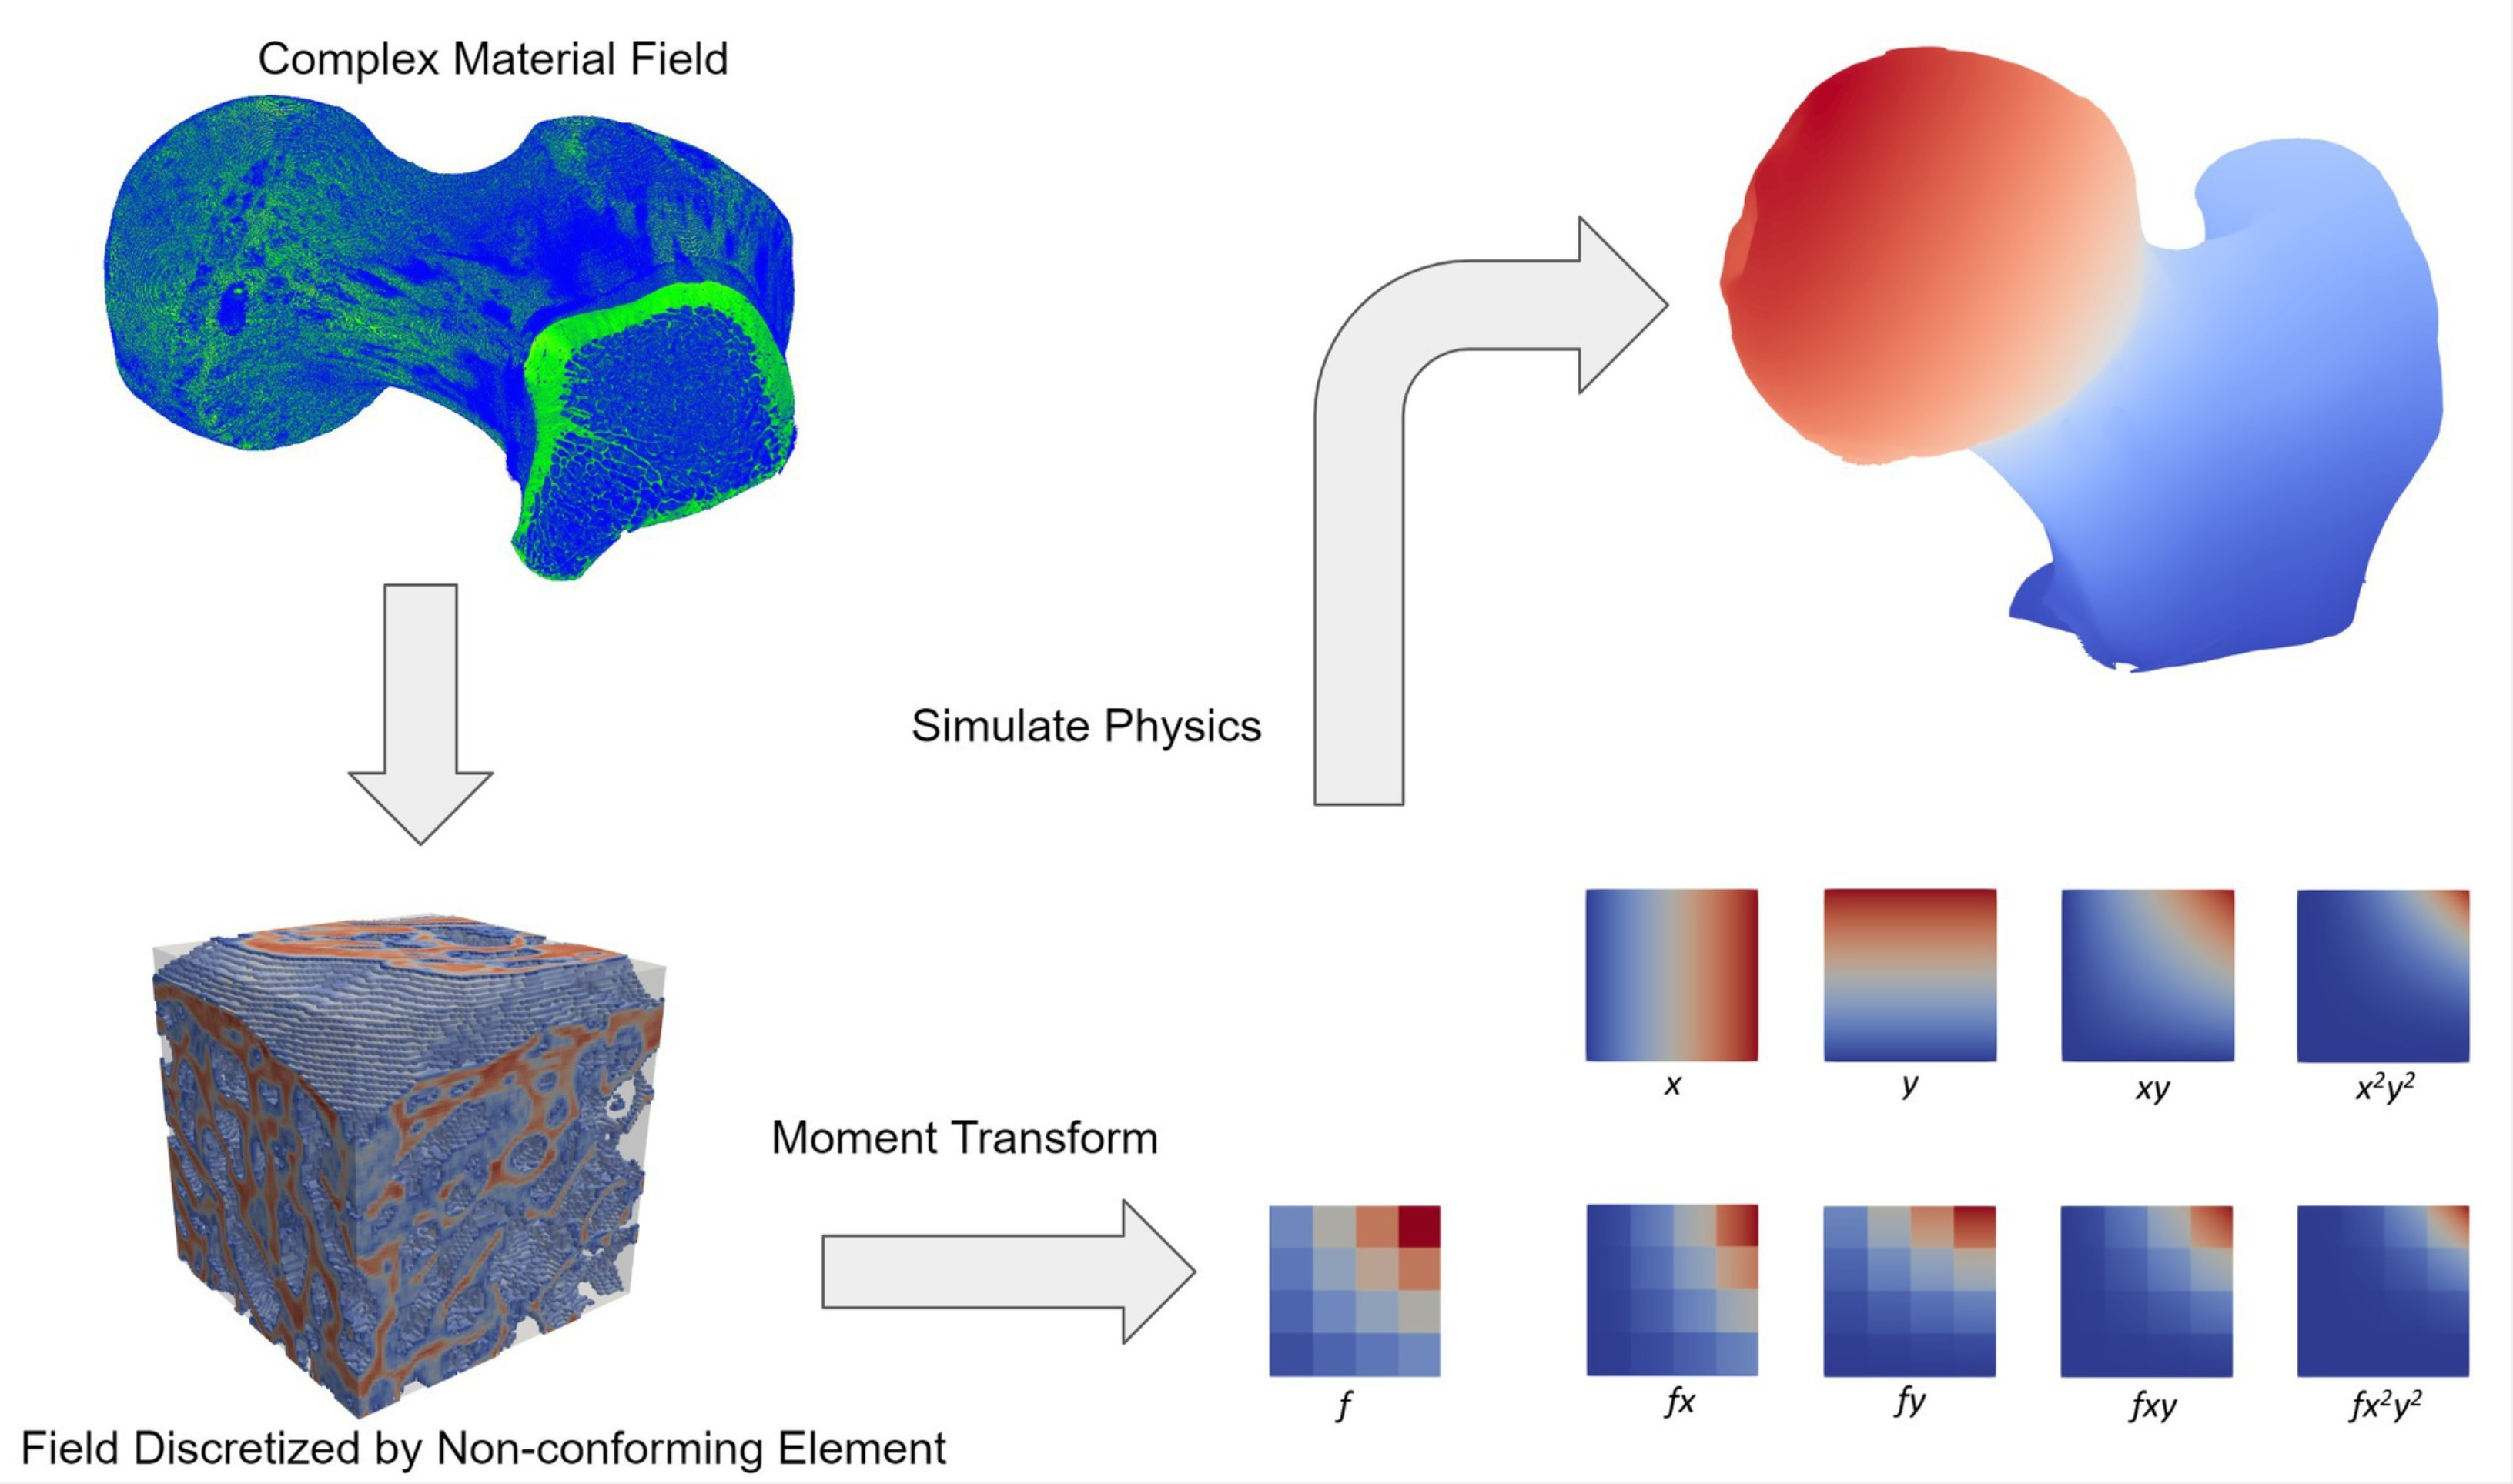
\includegraphics[width=0.8\linewidth]{bone_scan_example.png}\\
  \end{center}
    \blfootnote{Image from \cite{Taber2018}}
\end{frame}

\begin{frame}{Using the Divergence Theorem}
  \begin{center}
    \shadowimage[width=0.6\linewidth]{GeometryCell_scene_1.png}

    \shadowimage[width=0.3\linewidth]{GeometryCell_whole_1.png}
    \shadowimage[width=0.3\linewidth]{GeometryCell_outline_1.png}
  \end{center}
\end{frame}


\begin{frame}{Consequences}
\begin{columns}
\column{0.58\linewidth}
  \begin{outline}
    \1 Generalizes from just density to other fields like conductivity or even stiffness (spatially variable materials)
    \1 This was my job, shuttling data where it needs to be
  \end{outline}
\column{0.38\linewidth}
\begin{center}
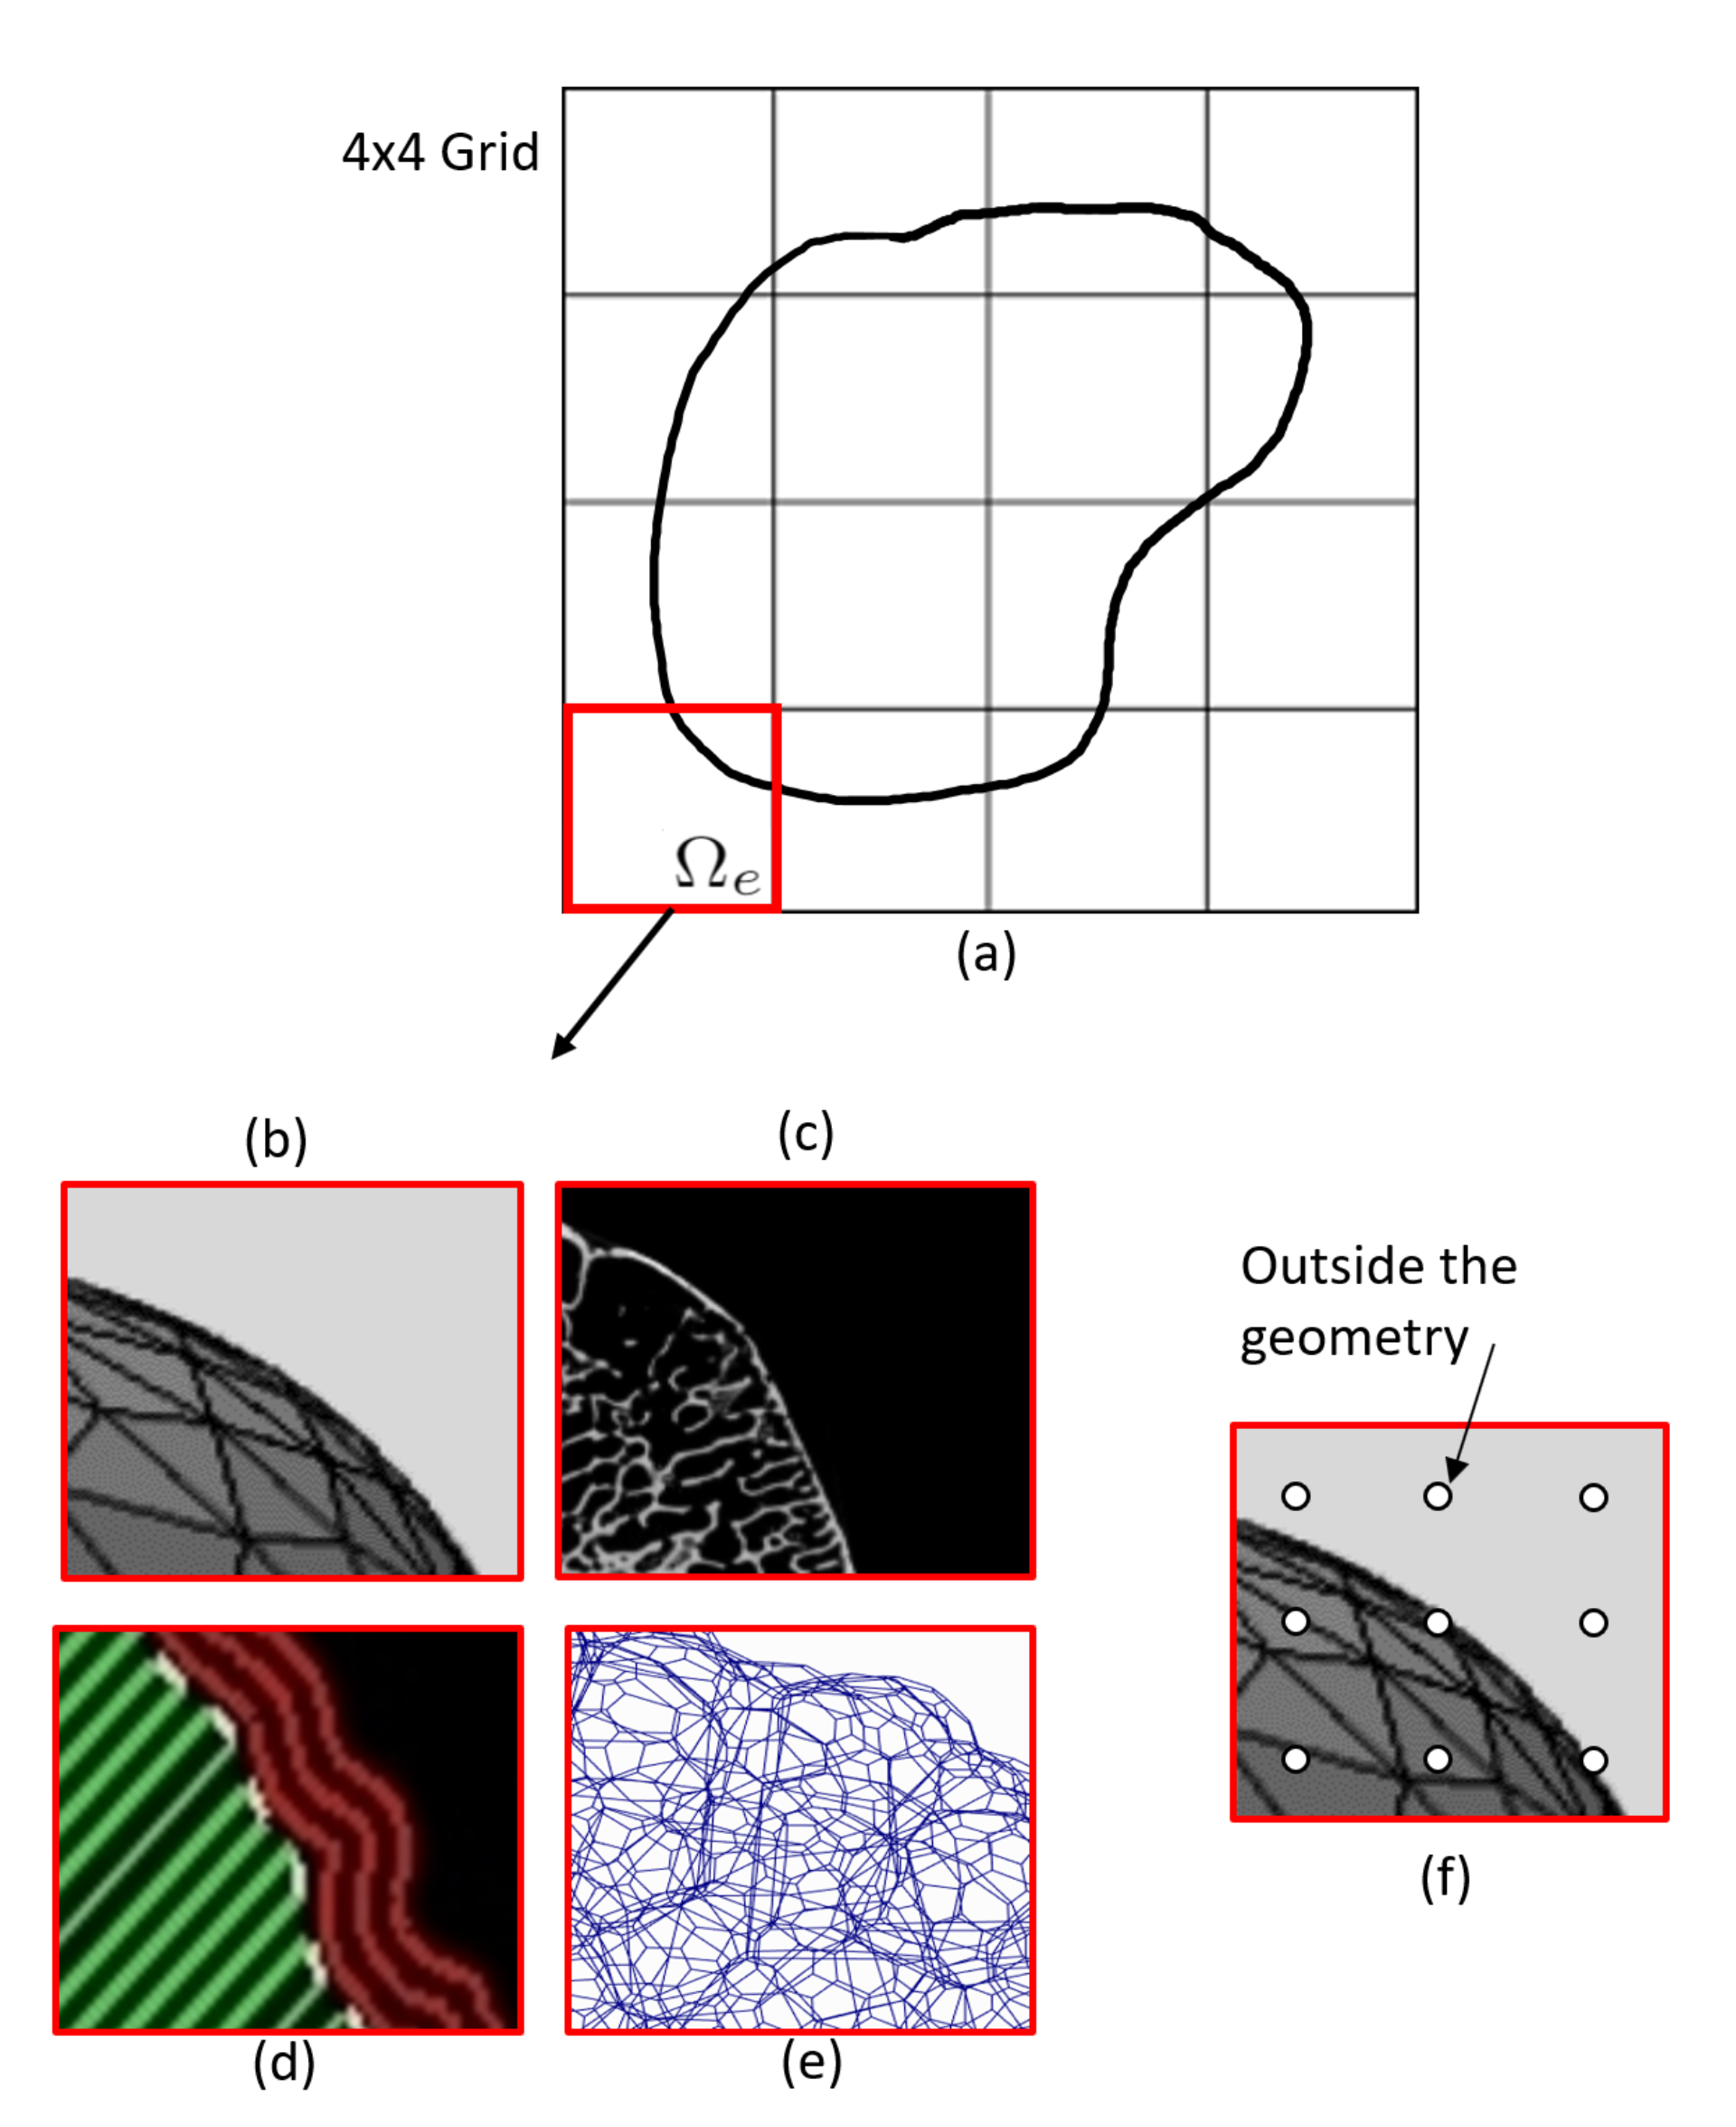
\includegraphics[width=4cm]{immersed_moments.png} 
\end{center}
\end{columns}
\blfootnote{Image from \cite{Taber2018}}
\end{frame}

